
\documentclass[a4paper, 12pt]{article}
\usepackage[portuguese]{babel}
\usepackage[utf8]{inputenc}
\usepackage[T1]{fontenc}
\usepackage{indentfirst}
\usepackage{graphicx}
\usepackage{listings}
\usepackage{color}
\usepackage{fancyhdr}
\usepackage{xfrac}
\usepackage{float}
\usepackage{geometry}
\usepackage{caption}
\usepackage{blindtext}
\usepackage{fullpage,supertabular,alltt,latexsym,amsfonts,/Users/renatonobre/Documents/.pvs/pvs/pvs}
\definecolor{mygreen}{RGB}{28,172,0}
\definecolor{mylilas}{RGB}{170,55,241}
\geometry{left=25mm, top=25mm, right=25mm, bottom=25mm}
\DeclareGraphicsExtensions{.pdf,.png,.jpg,.jpeg}
\captionsetup{labelformat=empty}

\lstset{language=Matlab,%
    %basicstyle=\color{red},
    breaklines=true,%
    morekeywords={matlab2tikz},
    keywordstyle=\color{blue},%
    morekeywords=[2]{1}, keywordstyle=[2]{\color{black}},
    identifierstyle=\color{black},%
    stringstyle=\color{mylilas},
    commentstyle=\color{mygreen},%
    showstringspaces=false,%without this there will be a symbol in the places where there is a space
    numbers=left,%
    numberstyle={\tiny \color{black}},% size of the numbers
    numbersep=9pt, % this defines how far the numbers are from the text
    emph=[1]{for,end,break},emphstyle=[1]\color{red}, %some words to emphasise
    %emph=[2]{word1,word2}, emphstyle=[2]{style},
}

\begin{document}
	\begin{titlepage}

		\newcommand{\HRule}{\rule{\linewidth}{0.5mm}}
		\centering
		\textsc{\LARGE Universidade de Brasília}\\[0.5cm]
		
\includegraphics{logo.jpg}\\[0.5cm]
		\textsc{\Large Instituto de Ciências Exatas}\\[0.5cm]
		\textsc{\Large Departamento de Ciência da Computação}\\[0.5cm]
		\textsc{\Large Princípios de Visão Computacional - Turma ``A''}\\[0.5cm]
		\HRule \\[0.4cm]
		{ \huge \bfseries Projeto Demonstrativo 2}\\[0.2cm]
		\HRule \\[3.0cm]
		\begin{minipage}{0.4\textwidth}
			\begin{flushleft} \large
				\emph{Nome:}\\
				\emph{Khalil Carsten}\\
				\emph{Renato Nobre}\\
			\end{flushleft}
		\end{minipage}
		~
		\begin{minipage}{0.4\textwidth}
			\begin{flushright} \large
				\emph{Matrícula:}\\
				\textsc{15/0134495}\\
				\textsc{15/0146698}\\
			\end{flushright}
		\end{minipage}\\[6.0cm]
		\textsc{\large \centering 4 de Setembro de 2017}\\
	\end{titlepage}

	\section*{Introdução}


    \section*{Desenvolvimento}
		\subsection*{Detecção dos pontos de interesse (SURF)}
        Como primeiro passo temos que detectar os pontos de interesse ou $features$ em
         todas as imagens, assim poderemos fazer uma comparação, entre esses pontos, nas imagens adjacentes.
        Devido a falta de uma implementação do algoritmo SIFT no MatLab utilizamos o SURF a partir da função:
        \\
        \begin{lstlisting}[frame=single]
detectSURFFeatures()
        \end{lstlisting}

        \begin{figure}[H]
            \centering
            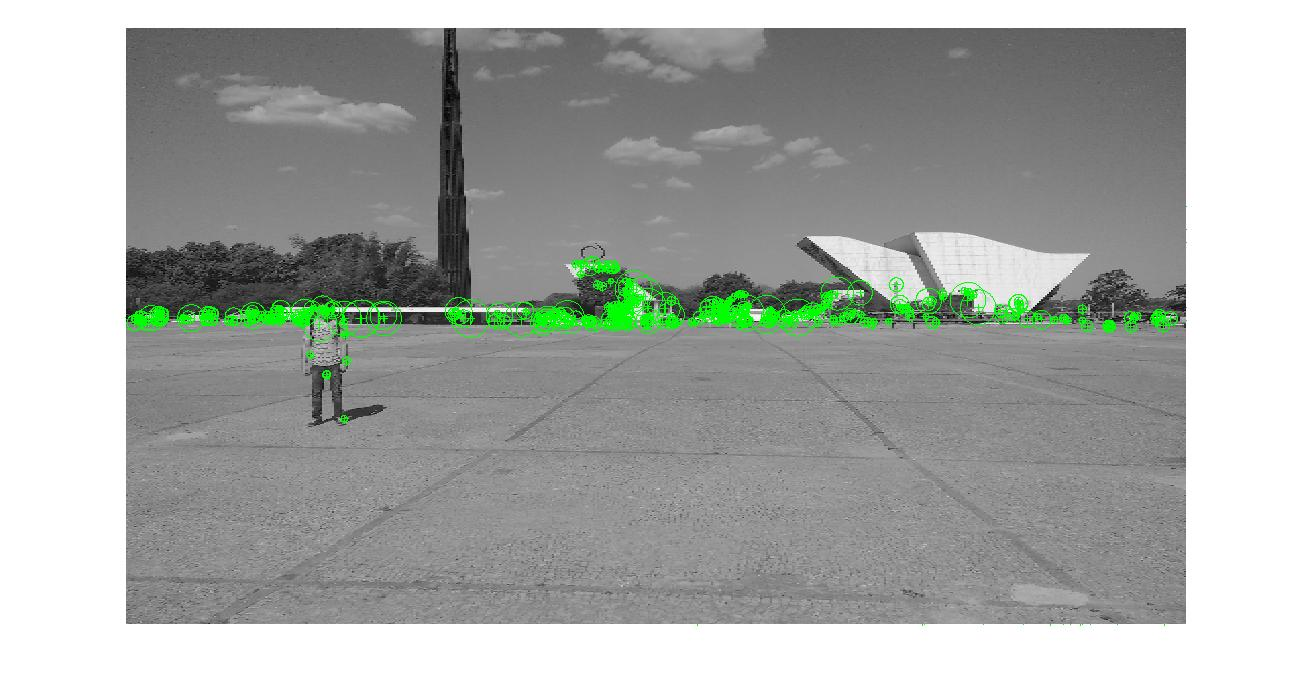
\includegraphics[width=1\linewidth]{SURF.jpg}
            \caption{Figura 1 - Exemplo visual da aplicação da detecção usando SURF.}
        \end{figure}

		\subsection*{Extraindo descritores e encontrando as distância entre seus pares}
        Como próximo passo precisamos extrair os descritores dos pontos de interesse, para isso
        utilizamos a função:

        \begin{lstlisting}[frame=single]
[features, points] = extractFeatures(I, points);
        \end{lstlisting}

        Mantendo em $features$ as características de cada ponto. Após isso precisamos calcular a distância
        entre cada 

		\begin{figure}[H]
			\centering
			\includegraphics[width=1\linewidth]{explication.jpg}
			\caption{Na imagem os nomes de cada segmento correspondem aos tamanhos calculados no código}
		\end{figure}

		Utilizamos a fórmula:
		$d = \sqrt {\left( {x_1 - x_2 } \right)^2 + \left( {y_1 - y_2 } \right)^2 }$
		para cálcular a distância entre os pontos.

		E para fazer a relação de proporcionalidade utilizamos outra fórmula:\\
		\\
		$tamRealDesejado = \frac{tamRealConhecido * Reta_1}{Reta_2}$
		\\
		\\
		Sendo $Reta_1$ e $Reta_2$ os tamanhos das retas na linha do horizonte representados como $Hinf$ e $Hlinf$ na imagem.
		\\
		A seguir econtra-se o código utilizado. O resultado final é armazanado na variável $altura2$.
		\begin{lstlisting}[frame=single]

  		\end{lstlisting}

	\subsection*{Fotos e Resultados da Altura Final}

	\subsection{Calculando a Matriz de Rotação}
	Para o Cálculo da matriz de rotação utilizamos um algoritmo de intersecção de retas, pois várias de nossa fotos ficaram impossíveis de calcular um segundo ponto de fuga manualmente.
	Então usamos a função $getline$ para obtermos as duas retas para o ponto de fuga e a fórmula:
	\\
	$x = -c_2*b_1 + c_1*b_2$
	\\
	$y = -c_1*b_2 + c_2*b_1$
	\\
	para encontrarmos o $x$ e o $y$ do ponto de intersecção entre elas.
	Seguindo o algoritmo passado no slide de "passo a passo" temos ao final $r_1$, $r_2$ e $r_3$.
	Como não tinhamos nenhum conhecimento sobre câmera utilizada mantivemos o valor mostrado na apresentação.
	Abaixo esta o código utilizado e as imagens nas quais conseguimos fazer a matriz de rotação e seus respectivos gráficos.
	\\
	\begin{lstlisting}[frame=single]
im = imread('Imagem5_linhas.jpg');
imshow(im);

% Le duas linhas para o ponto de fuga
ln1 = getline;
ln2 = getline;
% Le o ponto de fuga ja desenhado na tela
van1 = ginput(1);

% Cria a funcao da reta a partir de dois pontos
line1(1,1) = ln1(2,1) - ln1(1,1);
line1(1,2) = ln1(1,2) - ln1(2,2);
line1(1,3) = ln1(2,1)*ln1(1,2) - ln1(1,1)*ln1(2,2);

% Cria a funcao da reta a partir de dois pontos
line2(1,1) = ln2(2,1) - ln2(1,1);
line2(1,2) = ln2(1,2) - ln2(2,2);
line2(1,3) = ln2(2,1)*ln2(1,2) - ln2(1,1)*ln2(2,2);

% Calcula o determinante das duas retas
det = line1(1,1)*line2(1,2) - line1(1,2)*line2(1,1);

% Calcula a interseccao das duas retas
inter(1,1) = (-line2(1,3)*line1(1,2) + line1(1,3)*line2(1,2)) / det;
inter(1,2) = (-line1(1,3)*line2(1,1) + line2(1,3)*line1(1,1)) / det;

van2 = inter;

%foco
f = 1224;

%K
K = [f 0 size(im,2)/2;
     0 f size(im,1)/2;
     0 0 1];

% Atribuindo 1 a Z dos vanishing points
van1(1,3) = 1;
van2(1,3) = 1;


van1 = [van1(1,1);van1(1,2);van1(1,3)];
van2 = [van2(1,1);van2(1,2);van2(1,3)];

% Calculando r1 e r2
r1 = (inv(K)*van1)/norm(inv(K)*van1);
r2 = (inv(K)*van2)/norm(inv(K)*van2);

% Calculando r3
r3 = r1.*r2;

% Plota no grafico
plot3(r1, r2, r3);
	\end{lstlisting}

    \section*{Conclusão}
        O projeto realizado foi então validado comparando com a altura original das pessoas nas fotos a margem de erro é de aproximadamente 3 centímetros. A primeira pessoa que aparece nas duas primeiras imagens possui uma altura de $1.64$ metros, já a média da sua altura usando a altura encontrada nas as fotos foi de $1.61$ . Para a segunda pessoa, a média é de $1.72$, comparado com a altura real de $1.75$ metros.

        No entanto, o projeto apresenta certas dificuldades e limitações. Uma das principais dificuldades é em relação à disposição das fotos, que dependendo da maneira em que foi tirada pode se tornar impossível realizar os devidos cálculos. Outro ponto importante é que grande parte do projeto foi feito manualmente em vez de utilizar linhas de código para resolver o problema. Alguns passos podem ser automatizados, tais como, achar as linhas de fuga, o ponto de fuga, e detectar as pessoas nas imagens.

	\begin{thebibliography}{9}

        \bibitem{book1}
        Szeliski, Richard. ``Computer vision: algorithms and applications.'' Springer Science \& Business Media, 2010.

        \bibitem{slides}
        Slides de Aula


    \end{thebibliography}



\end{document}
